%!TEX root = ./recycling.tex
%
%

\section{Informal Development\label{sec:informal}}

We start by presenting our reasoning method informally for hazard pointers and
RCU, and illustrating the similarities between the two.

\subsection{Running Example}

%\begin{figure}[t]
%\begin{tabular}{@{\quad\ }l@{\quad}|@{\qquad}l@{}}
%{\small
%\begin{lstlisting}[numbers=left, numberstyle=\tiny,language=C,escapeinside={(*}{*)}]
%int *C = new int(0); (*\label{inc:gc:init}*)
%inc() {
%  int v, *s, *n;
%  n = new int; (*\label{inc:gc:alloc}*)
%  do {
%    s = C; (*\label{inc:gc:read}*)
%    v = *s; (*\label{inc:gc:deref}*)
%    *n = v+1; (*\label{inc:gc:store}*)
%  } while
%    (!CAS(&C, s, n));  (*\label{inc:gc:cas}*)
%  // free(s); (*\label{inc:gc:free}*)
%  return v;
%}
%\end{lstlisting}}
%&
%{\small
%\begin{lstlisting}[firstnumber=14,numbers=left, numberstyle=\tiny,language=C,escapeinside={(*}{*)}]
%int *C = new int(0);
%int *HP[N] = {0}; (*\label{inc:hp:HP}*)
%Set detached[N] = {(*$\emptyset$*)};(*\label{inc:hp:detached}*)
%int inc() {
%  int v, *n, *s, *s2;
%  n = new int;(*\label{inc:hp:alloc}*)
%  do {
%    do {
%      s = C; (*\label{inc:hp:readp}*)
%      HP[tid-1] = s; (* \label{inc:hp:sethp}*) 
%      s2 = C; (*\label{inc:hp:readpp}*)
%    } while (s != s2); (*\label{inc:hp:validate}*)
%    v = *s; (*\label{inc:hp:deref}*)
%    *n = v+1; (*\label{inc:hp:store}*)
%  } while(!CAS(&C, s, n)); (*\label{inc:hp:cas}*)
%  reclaim(s); (*\label{inc:hp:callretire}*)
%  return v; }
%\end{lstlisting}
%}
%\\[6pt]
%\qquad \qquad \quad {\small(a) } & \qquad \qquad \quad{\small (b)}
%\\[3pt]
%\end{tabular}
%\hrule
%\vspace{2pt}
%\begin{tabular}{@{\quad\ }l@{}}
%{\small
%\begin{lstlisting}[firstnumber=31,numbers=left, numberstyle=\tiny,language=C,escapeinside={(*}{*)}]
%void reclaim(int *s) {  
%  insert(detached[tid-1], s); (*\label{inc:hp:insretnew}*)
%  if (nondet()) return;
%  Set in_use = (*$\emptyset$*);
%  while (!isEmpty(detached[tid-1])) {
%    bool my = true;
%    int *n = pop(detached[tid-1]);    (*\label{inc:hp:pop}*)
%    for (int i = 0; i < N && my; i++) (*\label{inc:hp:checkhp1}*)
%      if (HP[i-1] == n) my = false; (*\label{inc:hp:checkhp2}*)
%    if (my) free(n); else insert(in_use, n); (*\label{inc:hp:free}*)
%  }
%  moveAll(detached[tid-1], in_use); }(*$\hspace{2cm}\mbox{\rm (c)}$*)(*\label{inc:hp:moveall}*)
%\end{lstlisting}
%}
%\end{tabular}
%%\\ 
%%\qquad\qquad \qquad (a) & \qquad \qquad \qquad (b) & \qquad \qquad \qquad \qquad
%%\quad(c)
%\caption{A shared counter: (a) an implementation leaking memory; (b)-(c) an
%  implementation based on hazard pointers. {\tt tid} gives the identifier of the
%  current thread.}
%\label{fig:running}
%\end{figure}

\begin{figure}[t]
%\begin{tabular}{@{\quad\ }l@{\quad}|@{\qquad}l@{}}
\begin{tabular}{@{\quad\ }l@{}|@{\quad\ }l@{}|@{\quad\ }l@{}}
{\figfontsize
\begin{lstlisting}[numbers=left, numberstyle=\tiny,language=C,escapeinside={(*}{*)}]
int *C = new int(0); (*\label{inc:gc:init}*)
int inc() {
  int v, *s, *n;
  n = new int; (*\label{inc:gc:alloc}*)
  do {
    s = C; (*\label{inc:gc:read}*)
    v = *s; (*\label{inc:gc:deref}*)
    *n = v+1; (*\label{inc:gc:store}*)
  } while
    (!CAS(&C,s,n));  (*\label{inc:gc:cas}*)
  // free(s); (*\label{inc:gc:free}*)
  return v;
}
\end{lstlisting}}
&
{\figfontsize
\begin{lstlisting}[firstnumber=14,numbers=left, numberstyle=\tiny,language=C,escapeinside={(*}{*)}]
int *C = new int(0);
int *HP[N] = {0}; (*\label{inc:hp:HP}*)
Set detached[N] = {(*$\emptyset$*)};(*\label{inc:hp:detached}*)
int inc() {
  int v, *n, *s, *s2;
  n = new int;(*\label{inc:hp:alloc}*)
  do {
    do {
      s = C; (*\label{inc:hp:readp}*)
      HP[tid-1] = s; (* \label{inc:hp:sethp}*) 
      s2 = C; (*\label{inc:hp:readpp}*)
    } while (s != s2); (*\label{inc:hp:validate}*)
    v = *s; (*\label{inc:hp:deref}*)
    *n = v+1; (*\label{inc:hp:store}*)
  } while(!CAS(&C,s,n)); (*\label{inc:hp:cas}*)
  reclaim(s); (*\label{inc:hp:callretire}*)
  return v; }
\end{lstlisting}
}
&
%\\[6pt]
%\qquad \qquad \quad {\small(a) } & \qquad \qquad \quad{\small (b)}
%\\[3pt]
%\end{tabular}
%\hrule
%\vspace{2pt}
%\begin{tabular}{@{\quad\ }l@{}}
{\figfontsize
\begin{lstlisting}[firstnumber=31,numbers=left, numberstyle=\tiny,language=C,escapeinside={(*}{*)}]
void reclaim(int *s) {  
  insert(detached[tid-1],s); (*\label{inc:hp:insretnew}*)
  if (nondet()) return;
  Set in_use = (*$\emptyset$*);
  while (!isEmpty(
      detached[tid-1])) {
    bool my = true;
    int *n = 
      pop(detached[tid-1]);    (*\label{inc:hp:pop}*)
    for (int i = 0; (*\label{inc:hp:checkhp1}*)
        i < N && my; i++) 
      if (HP[i] == n) 
        my = false; (*\label{inc:hp:checkhp2}*)
    if (my) free(n); (*\label{inc:hp:free}*)
    else insert(in_use, n); 
  }
  moveAll(detached[tid-1], 
    in_use); }(*\label{inc:hp:moveall}*)
\end{lstlisting}
}
\\[6pt]
\qquad\qquad (a) & \qquad \qquad \quad (b) & \qquad \qquad \quad 
\quad(c)
%\qquad \qquad \quad {\small(a) } & \qquad \qquad \quad{\small (b)}
\end{tabular}
%\\ 
%\qquad\qquad \qquad (a) & \qquad \qquad \qquad (b) & \qquad \qquad \qquad \qquad
%\quad(c)
\caption{\small A shared counter: (a) an implementation leaking memory; (b)-(c) an
  implementation based on hazard pointers. Here {\tt tid} gives the identifier of the
  current thread.}
\label{fig:running}
\end{figure}


As our running example, we use a counter with an increment operation {\tt inc}
that can be called concurrently by multiple threads. Despite its simplicity, the
example is representative of the challenges that arise when reasoning about
more complex algorithms.

%concurrent data structures with memory reclamation.

The implementation shown in Figure~\ref{fig:running}a follows a typical pattern
of non-blocking algorithms.  The current value of the counter is kept in a
heap-allocated node pointed to by the global variable $\cc$.  To increment the
counter, we allocate a new memory cell {\tt n} (line~\ref{inc:gc:alloc}),
atomically read the value of $\cc$ into a local pointer variable \texttt{s}
(line~\ref{inc:gc:read}), dereference \texttt{s} to get the value \texttt{v} of
the counter (line~\ref{inc:gc:deref}), and then store \texttt{v}'s successor
into {\tt n} (line~\ref{inc:gc:store}).  At that point, we try to change $\cc$
so that it points to {\tt n} using an atomic \emph{compare-and-swap} (CAS)
command (line~\ref{inc:gc:cas}). A CAS takes three arguments: a memory address
(e.g., \verb|&C|), an expected value ({\tt s}) and a new value ({\tt n}). It
atomically reads the memory address and updates it with the new value if the
address contains the expected value; otherwise, it does nothing. The CAS thus
succeeds only if the value of $\cc$ is the same as it was when we read it at
line~\ref{inc:gc:read}, thus ensuring that the counter is updated correctly. If
the CAS fails, we repeat the above steps all over again.
%
% \begin{source}
%   atomic { 
%     if (*addr==v1) { *addr=v2; return 1; } 
%     else { return 0; } 
%   }
% \end{source}
%
The algorithm is \emph{memory safe}, i.e., it never accesses unallocated memory
cells. It is also functionally correct in the sense that every increment
operation appears to take effect atomically.  More formally, the counter is
\emph{linearizable} with respect to the expected sequential counter
specification~\cite{linearizability}. Unfortunately, the algorithm leaks memory,
as the node replaced by the CAS is never reclaimed. It is thus not appropriate
for %run-time 
environments without garbage collection.
 
\paragraph{A naive fix.} One can try to prevent memory leakage by uncommenting
the {\tt free} command in line~\ref{inc:gc:free} of Figure~\ref{fig:running}a,
so that the node previously pointed to by $\cc$ is deallocated by the thread
that changed $\cc$'s value (in this case we say that the thread {\em
  detached} the node). However, this violates both memory safety and
linearizability. To see the former, consider two concurrent threads, one of
which has just read the value $x$ of $\cc$ at line~\ref{inc:gc:read}, when the
other executed {\tt inc} to completion and reclaimed the node at the address
$x$. When the first thread resumes at line~\ref{inc:gc:deref} it will access an
unallocated memory cell.

The algorithm also has executions where a memory fault does not happen, but {\tt
  inc} just returns an incorrect value. Consider the following scenario: a
thread $t_1$ running \texttt{inc} gets preempted after executing
line~\ref{inc:gc:deref} and, at that time, $\cc$ points to a node $x$ storing
$v$; a thread $t_2$ executes \texttt{inc}, deallocating the node $x$
and incrementing the counter to $v+1$; a thread $t_3$ calls {\tt inc} and
allocates $x$, recycled by the memory system; $t_3$ stores $v+2$ into $x$ and
makes $\cc$ point to it; $t_1$ wakes up, its CAS succeeds, and it sets the
counter value to $v+1$, thereby decrementing it!
This is a particular instance of the well-known {\em ABA
  problem}: if we read the value $A$ of a global variable and later check
that it has the value $A$, we cannot conclude, in general, 
that in the meantime it did not change to another value $B$ and then back to $A$.  
The version of the algorithm without {\tt free} in line~\ref{inc:gc:free} does
not suffer from this problem, as it always allocates a fresh cell. 
This algorithm is also correct when executed in a
garbage-collected environment, as in this case the node $x$ in the above
scenario will not be recycled as long as $t_1$ keeps the pointer {\tt s}
to it.


\subsection{Reasoning about Hazard Pointers}

Figure~\ref{fig:running}b shows a correct implementation of {\tt inc} with
explicit memory reclamation based on {\em hazard pointers}~\cite{hazard}. We
assume a fixed number of threads with identifiers from $1$ to $\nthreads$. As
before, the thread that detaches a node is in charge of reclaiming it.  However,
it delays the reclamation until it is assured that no other thread requested
that the node be protected from reclamation. A thread announces a request for a
node to be protected using the array \texttt{HP} of shared hazard pointers
indexed by thread identifiers.  Every thread is allowed to write to the entry in
the array corresponding to its identifier and read all entries. To protect
the location {\tt s}, a thread writes {\tt s} into its entry of the hazard array
(line~\ref{inc:hp:sethp}) and then checks that the announcement was not too late
by validating that \texttt{C} still points to {\tt s}
(line~\ref{inc:hp:validate}).  Once the validation succeeds, the thread is
assured that the node {\tt s} will not be deallocated as long as it keeps its
hazard pointer equal to {\tt s}. In particular, it is guaranteed that
the node {\tt s} remains allocated when executing lines
\ref{inc:hp:deref}--\ref{inc:hp:cas}, which ensures that the algorithm is memory
safe.  This also guarantees that, if the CAS in line \ref{inc:hp:cas} is
successful, then $\cc$ has not changed its value since the thread read it at
line~\ref{inc:hp:readpp}. This prevents the ABA problem and makes the algorithm
linearizable.

The protection of a node pointed to by a hazard pointer is ensured by the
behaviour of the thread that detaches it. Instead of invoking {\tt free}
directly, the latter uses the \texttt{reclaim} procedure in
Figure~\ref{fig:running}c. This stores the node in a thread-local {\tt detached}
set (line~\ref{inc:hp:insretnew}) and occasionally performs a batched
reclamation from this set (for clarity, we implemented {\tt detached} as an
abstract set, rather than a low-level data structure). To this end,
the thread considers every node {\tt n} from the set and checks that no hazard
pointer points to it (lines~\ref{inc:hp:checkhp1}--\ref{inc:hp:checkhp2}).  If
the check succeeds, the node gets deallocated (line~\ref{inc:hp:free}).


\paragraph{Reasoning challenges.}
The main idea of hazard pointers is simple: threads accessing the shared data
structure set hazard pointers to its nodes, and threads reclaiming memory check
these pointers before deallocating nodes. However, the mechanics of implementing
this protocol in a non-blocking way is very subtle. 

For example, when a thread $t_1$ deallocates a node $x$ at
line~\ref{inc:hp:free}, we may actually have a hazard pointer of another thread
$t_2$ pointing to $x$. This can occur in the following scenario: $t_2$ reads the
address $x$ from $\cc$ at line~\ref{inc:hp:readp} and gets preempted; $t_1$'s CAS
detaches $x$ and successfully passes the check in
lines~\ref{inc:hp:checkhp1}--\ref{inc:hp:checkhp2}; $t_2$ wakes up and sets its
hazard pointer to $x$; $t_1$ deallocates $x$ at line~\ref{inc:hp:free}. However,
such situations do not violate the correctness, as the next thing $t_2$ will do
is to check that $\cc$ still points to $x$ at line~\ref{inc:hp:validate}.  Provided
$x$ has not yet been recycled by the memory system, this check will fail and the
hazard pointer of $t_2$ will have no force. This shows that the additional check
in line~\ref{inc:hp:validate} is indispensable for the algorithm to be correct.

It is also possible that, before $t_2$ performs the check in
line~\ref{inc:hp:validate}, $x$ is recycled, allocated at
line~\ref{inc:hp:alloc} by another thread $t_3$ and inserted into the shared
data structure at line~\ref{inc:hp:cas}. In this case, the check by $t_2$
succeeds, and the element can safely be accessed. This highlights
a subtle point: when $t_3$ executes the CAS at
line~\ref{inc:hp:cas} to insert $x$, we might already have a hazard pointer
pointing to $x$. This, however, does not violate correctness.

\paragraph{Our approach.}
We achieve a % simple and 
natural reasoning about hazard pointers and similar
patterns by formalising the main intuitive concept in their design---that of a
{\em grace period}. As follows from the above explanation, a thread $t$ can only
be sure that a node $x$ its hazard pointer points to is not deallocated after a
moment of time when both the hazard pointer was set and the node was pointed to
by $\cc$. The grace period for the node $x$ and thread $t$ starts from this
moment and lasts for as long as the thread keeps its hazard pointer pointing to
$x$. Informally, this is described by the following  temporal judgement:
\be\label{inf-grace} \mbox{
\begin{minipage}{10cm}
``the hazard pointer of thread $t$ has pointed to $x$ \underline{since}
  $\cc$ pointed to $x$'',
\end{minipage}
}
\ee
where \underline{since} is a temporal connective with the expected
interpretation: both of the facts connected were true at some point,
and since then, the first fact has stayed true. We can thus specify the contract
between threads accessing  nodes and those trying to reclaim them by the
following invariant that all threads have to respect:
\be\label{inf-inv} \mbox{
\begin{minipage}{10cm}
  ``for all $t$ and $x$, if the hazard pointer of thread $t$ has pointed to $x$
  \underline{since} $\cc$ pointed to $x$, then $x$ is allocated.''
\end{minipage}
}
\ee

It is this invariant that justifies the safety of the access to a shared node
at line~\ref{inc:hp:deref}. On the other hand, a thread that wants to deallocate
$x$ when executing {\tt reclaim} checks that the hazard pointers of other
threads do not point to $x$ 
(lines~\ref{inc:hp:checkhp1}--\ref{inc:hp:checkhp2}) only after detaching the node
from the shared data structure, and it keeps the node in the {\tt detached} set until
its deallocation. Thus, even though threads can set their hazard pointers to $x$
after the reclaimer executes the check in
lines~\ref{inc:hp:checkhp1}--\ref{inc:hp:checkhp2}, they cannot do this at the
same time as $\cc$ points to $x$. Hence, when the reclaimer deallocates $x$ at
line~\ref{inc:hp:free}, we know that
\be\label{inf-neg} \mbox{
\begin{minipage}{10cm}
  ``for all $t$, $\cc$ has not pointed to $x$ \underline{since} the hazard
  pointer of $t$ did not point to $x$.''
\end{minipage}
} \ee 
%It is easy to see that this  
Clearly, (\ref{inf-neg})  
is inconsistent with~(\ref{inf-grace}). Therefore,
no thread is inside a grace period for $x$ at the time of its deallocation, and
the command in line~\ref{inc:hp:free} does not violate % the
invariant~(\ref{inf-inv}).

More formally, let us denote the property ``the hazard pointer of thread $t$
points to node $x$'' by $\eta_{t,x}$, ``$\cc$ points to node $x$'' by $\mu_x$, and
``$x$ is allocated'' by $\lambda_x$. Then (\ref{inf-grace}) is $(\eta_{t, x} \since
\mu_x)$, (\ref{inf-inv}) is $(\forall t, x.\, (\eta_{t, x} \since \mu_x) {\implies}
\lambda_x)$, and (\ref{inf-neg}) is $(\forall t.\, \neg \mu_x \since \neg \eta_{t,x})$. The
combination of~(\ref{inf-grace}) and~(\ref{inf-neg}) is inconsistent due to the
following tautology: % in temporal logic:
\be\label{incons}
\forall \eta,\mu.\,
(\eta \since \mu) \wedge (\neg \mu \since \neg \eta) \implies \false.
\ee

The above argument justifies the memory safety of the algorithm, and (as we show
in \S\ref{sec:grace}) the absence of memory leaks. Moreover,~(\ref{inf-inv})
guarantees to a thread executing {\tt inc} that, when the CAS in
line~\ref{inc:hp:cas} succeeds, the node {\tt s} has not been reallocated, and
so the ABA problem does not occur.

We have achieved a simple reasoning about the algorithm by defining the duration
of a grace period~(\ref{inf-grace}), the protocol all threads
follow~(\ref{inf-inv}), and the fact a reclaimer establishes before deallocating
a node~(\ref{inf-neg}) as temporal formulas of particular forms. We find that
the above reasoning with temporal facts of these forms is applicable not only to
our example, but also to uses of hazard pointers in other data structures
\tra{\ref{sec:ProofsHazard}}{\nhazard}, and in fact, to completely different
approaches to memory reclamation, as we now illustrate.



\subsection{Reasoning about Read-Copy-Update\label{sec:rcu-prelim}}

Read-Copy-Update (RCU)~\cite{rcu-thesis} is a non-standard synchronisation
mechanism used in Linux to ensure safe memory deallocation in data structures
with concurrent access. So far, there have been no methods for reasoning about
programs with RCU. We now show that we can use our temporal reasoning principle
based on grace periods to this end.

%RCU is widely used in Linux, where it achieves efficiency by piggy-backing on
%the scheduler implementation.



%that allows multiple threads to coordinate accesses to a shared data structure
%efficiently.



\paragraph{RCU primer.}
RCU provides three commands: $\rlock$, $\runlock$ and
$\sync$. The $\rlock$ and $\runlock$ commands delimit an RCU {\em critical
  section}. They do {\em not} ensure mutual exclusion, so multiple
threads can be in their critical sections simultaneously. Instead of enforcing
mutual exclusion, RCU provides the $\sync$ command, which records the
identifiers of the threads currently in critical sections and waits until all of
them exit the sections. Note that if a new thread enters a critical section
while $\sync$ is waiting, the command does not wait for the completion of its
section. For example, when $t_1$ calls $\sync$ in the execution in
Figure~\ref{fig:timeline}, it has to wait for critical sections $S_1$, $S_5$ and
$S_6$ to finish. However, it does not wait for %sections 
$S_2$ or $S_4$, as they
start after $\sync$ was called.


\begin{figure}[t]
\begin{tabular}{@{\quad\ }l@{;}r@{}}
\begin{minipage}{0.5\textwidth}
{\figfontsize
\begin{lstlisting}[numbers=left, numberstyle=\tiny, language=C, escapeinside={(*}{*)}]
bool rcu[N] = {0};
rcu_enter() {(*$\langle$*)rcu[tid-1]=1(*$\rangle_{\textsf{RCU}_\tid}$*);} 
rcu_exit() {(*$\langle$*)rcu[tid-1]=0(*$\rangle_{\textsf{RCU}_\tid}$*);} 
sync() {
  bool r[N] = {0};
  for(int i = 0; i < N; i++) 
    (*$\langle$*)r[i] = rcu[i](*$\rangle_{\textsf{Id}}$\label{impl:snap}*);
  for(int i = 0; i < N; i++) (*\label{impl:wait2}*)
    if(r[i]) {while((*$\langle$*)rcu[i](*$\rangle_{\textsf{Id}}$\label{impl:wait}*));}
}
\end{lstlisting}
}
\end{minipage}
&
\!\!\!\!\!\!\!\!\!\!\!\!\!\!\!\!\!\!\!
\begin{minipage}{0.63\textwidth}
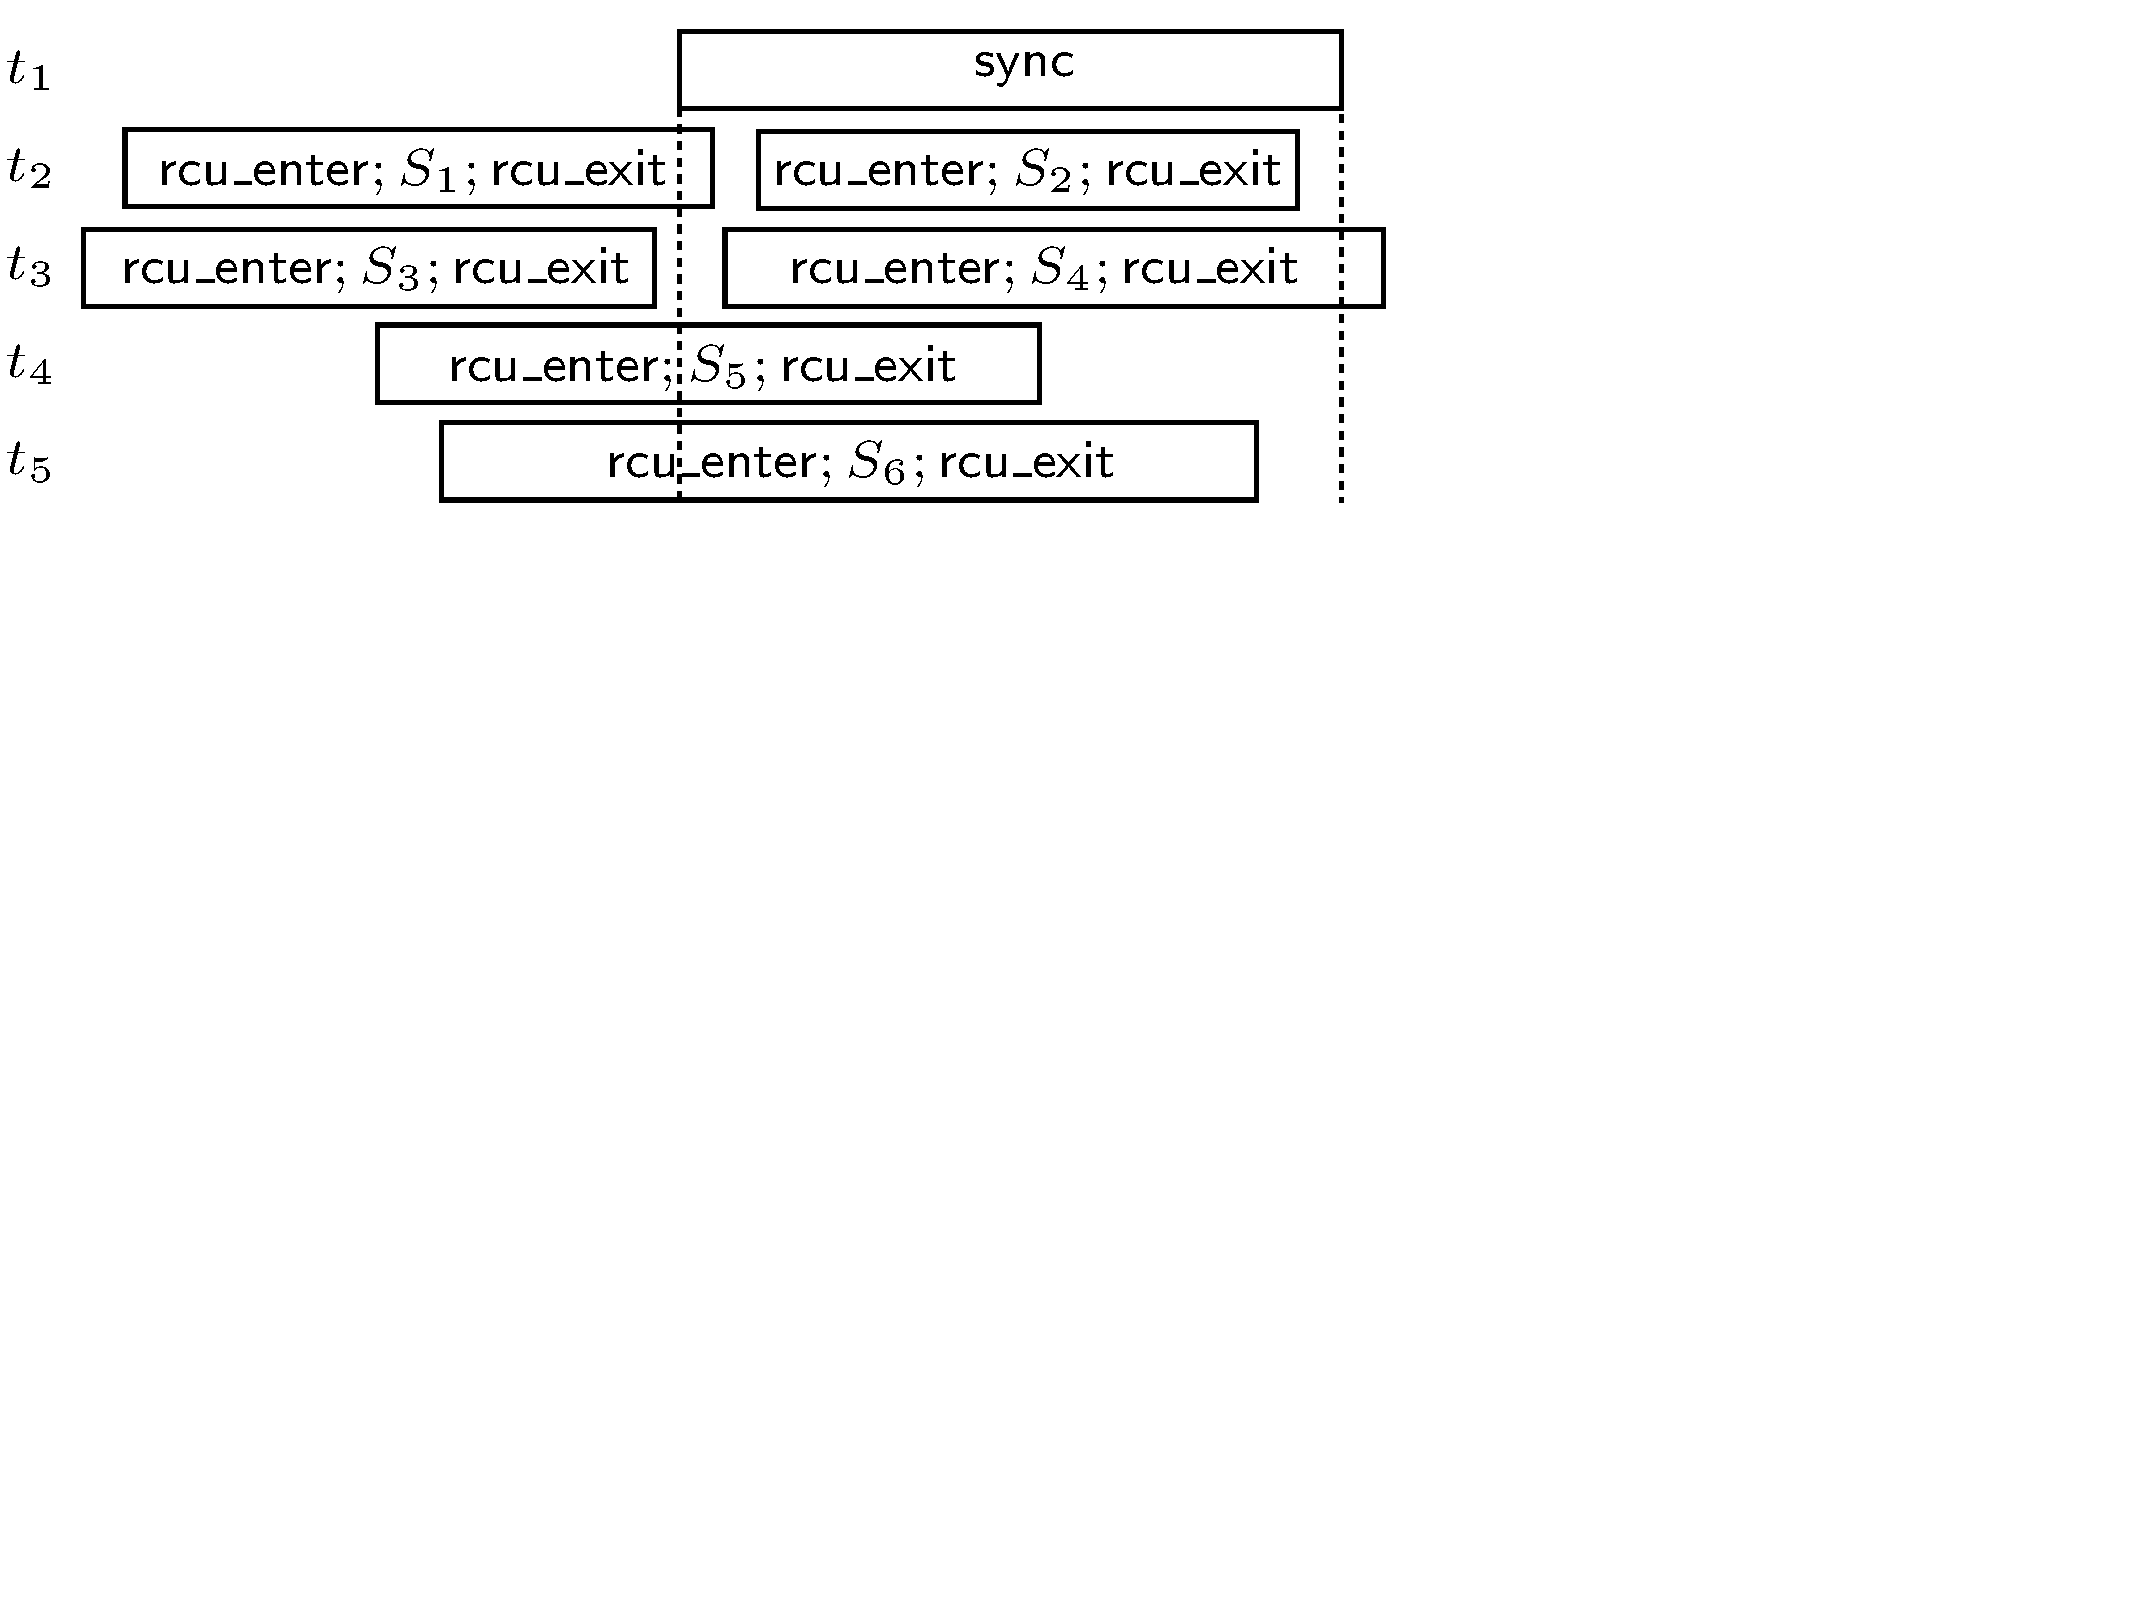
\includegraphics[scale=.275, trim= 0 18.5cm 0 0.1cm]{sync}
\end{minipage}
\end{tabular}
 \caption{\small An abstract RCU implementation and an illustration of the semantics of $\sync$. 
  Blocks represent the time spans of RCU critical sections or an execution of $\sync$.}
\label{fig:timeline}\label{fig:RCUProofSketch} 
\end{figure}

%%\begin{minipage}
%\begin{figure}[t]
%%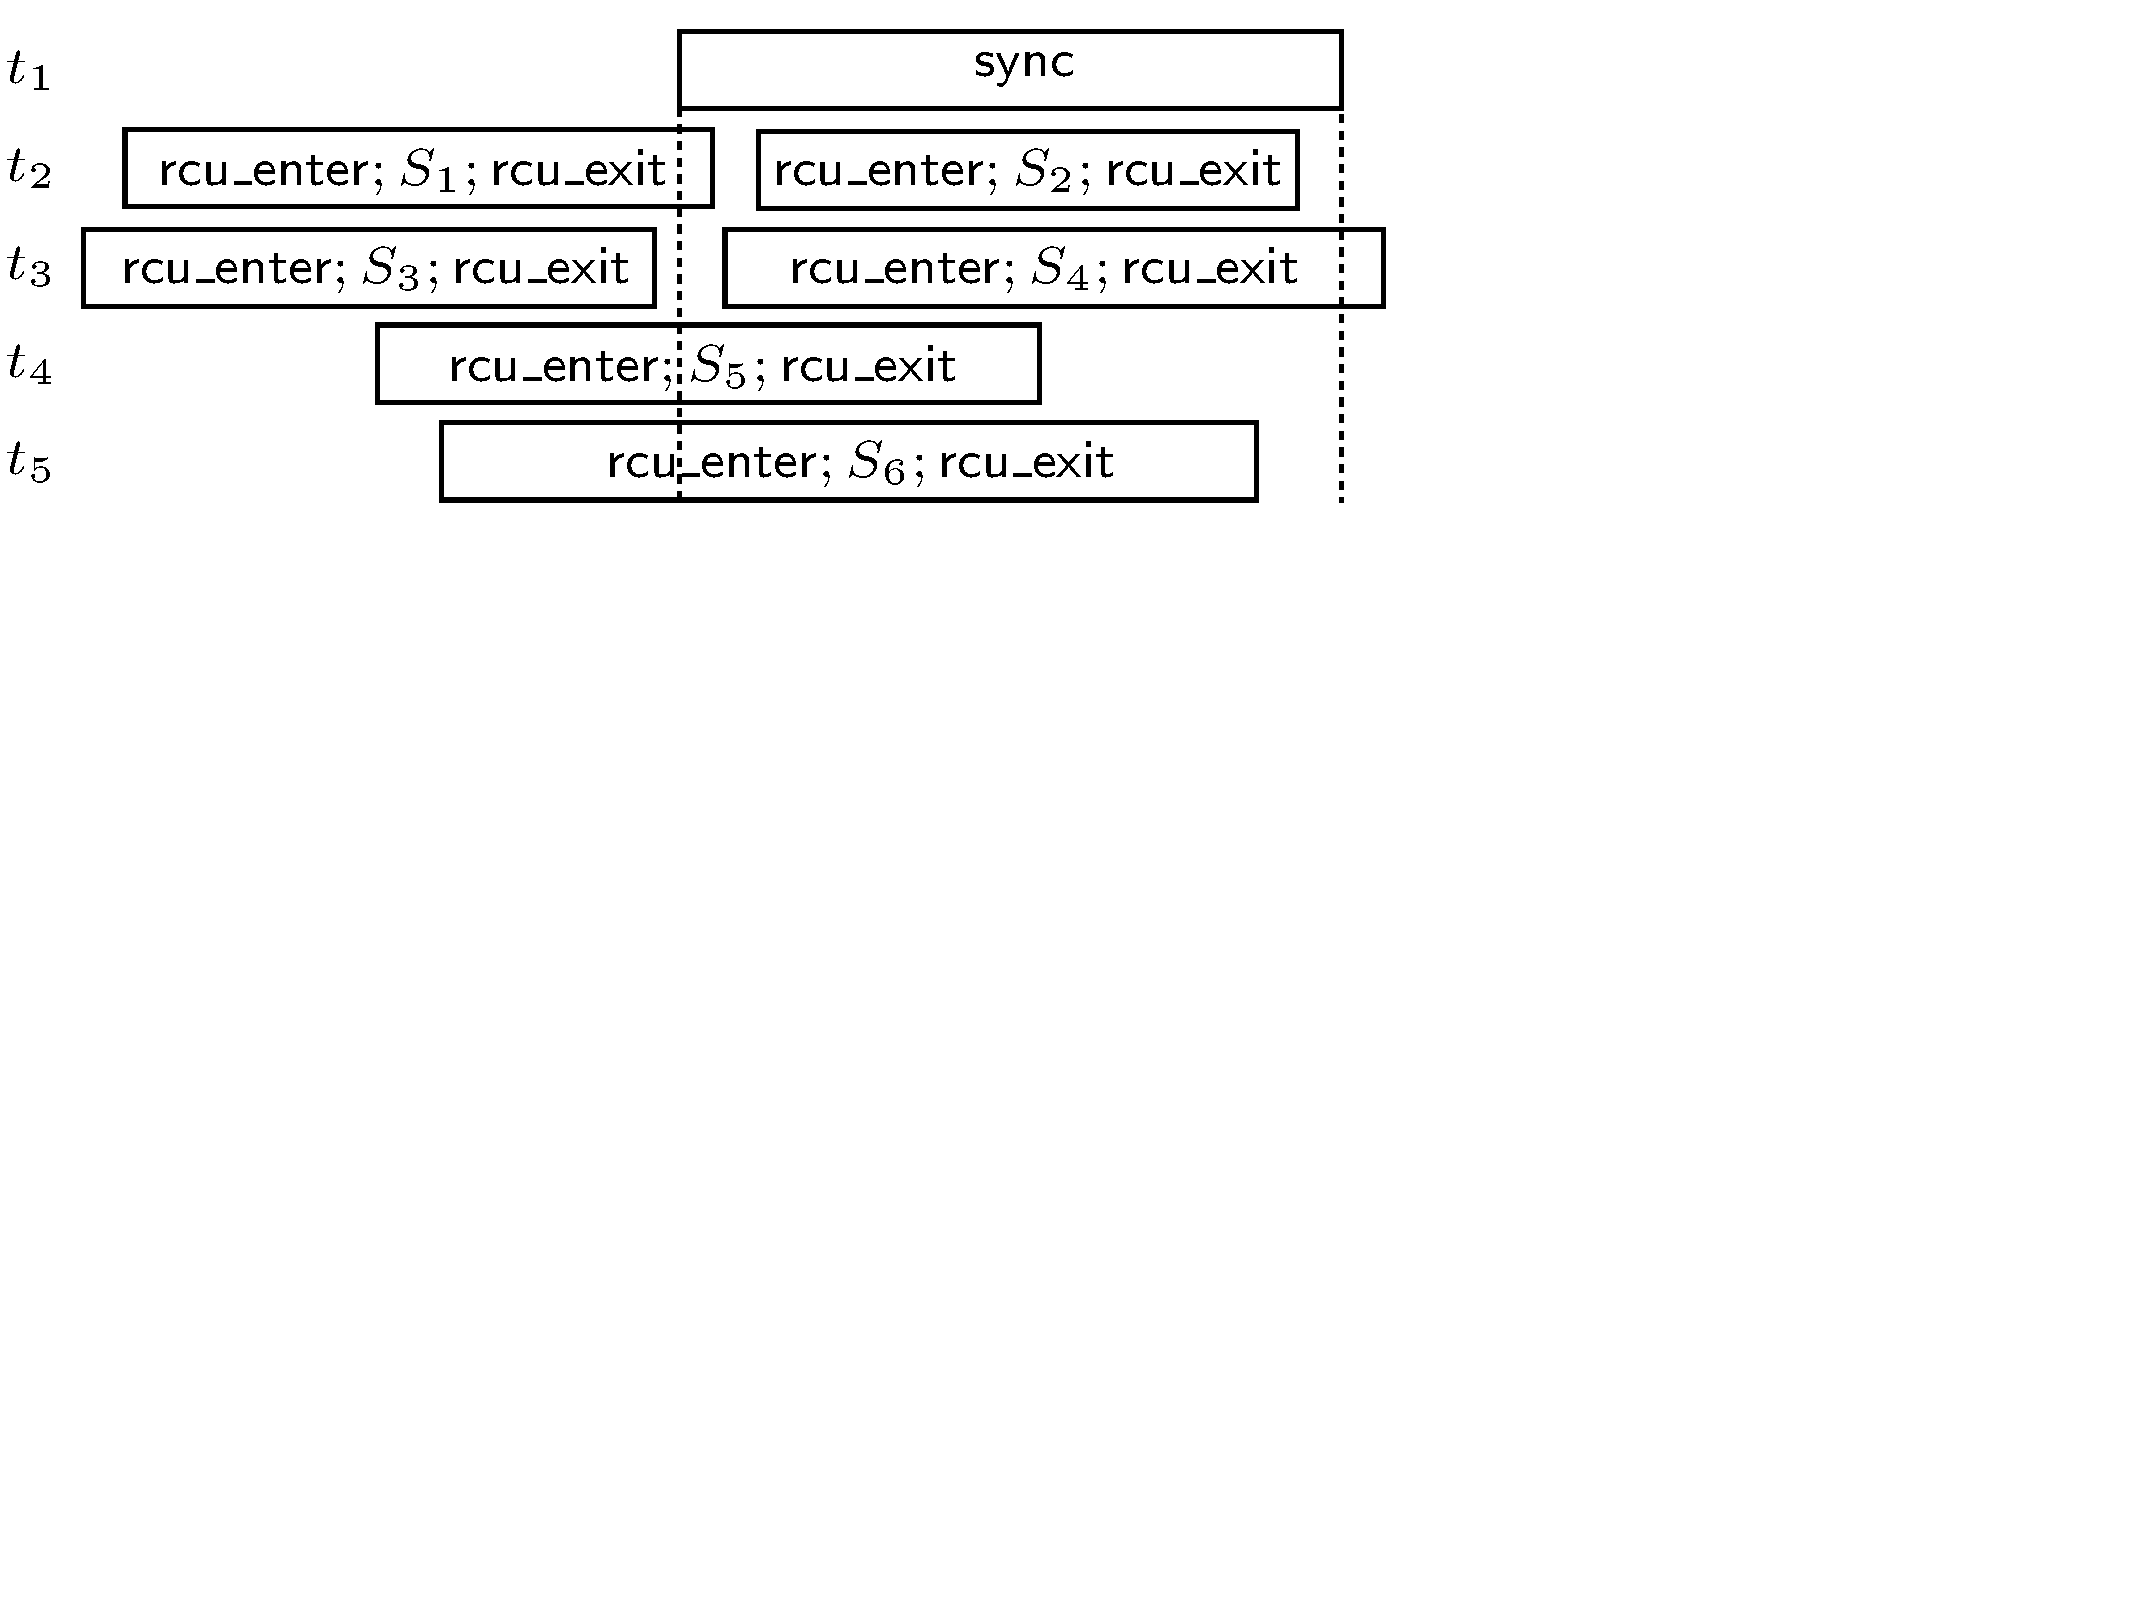
\includegraphics[scale=.25, trim= 0 19.2cm 0 0.1cm]{sync}
%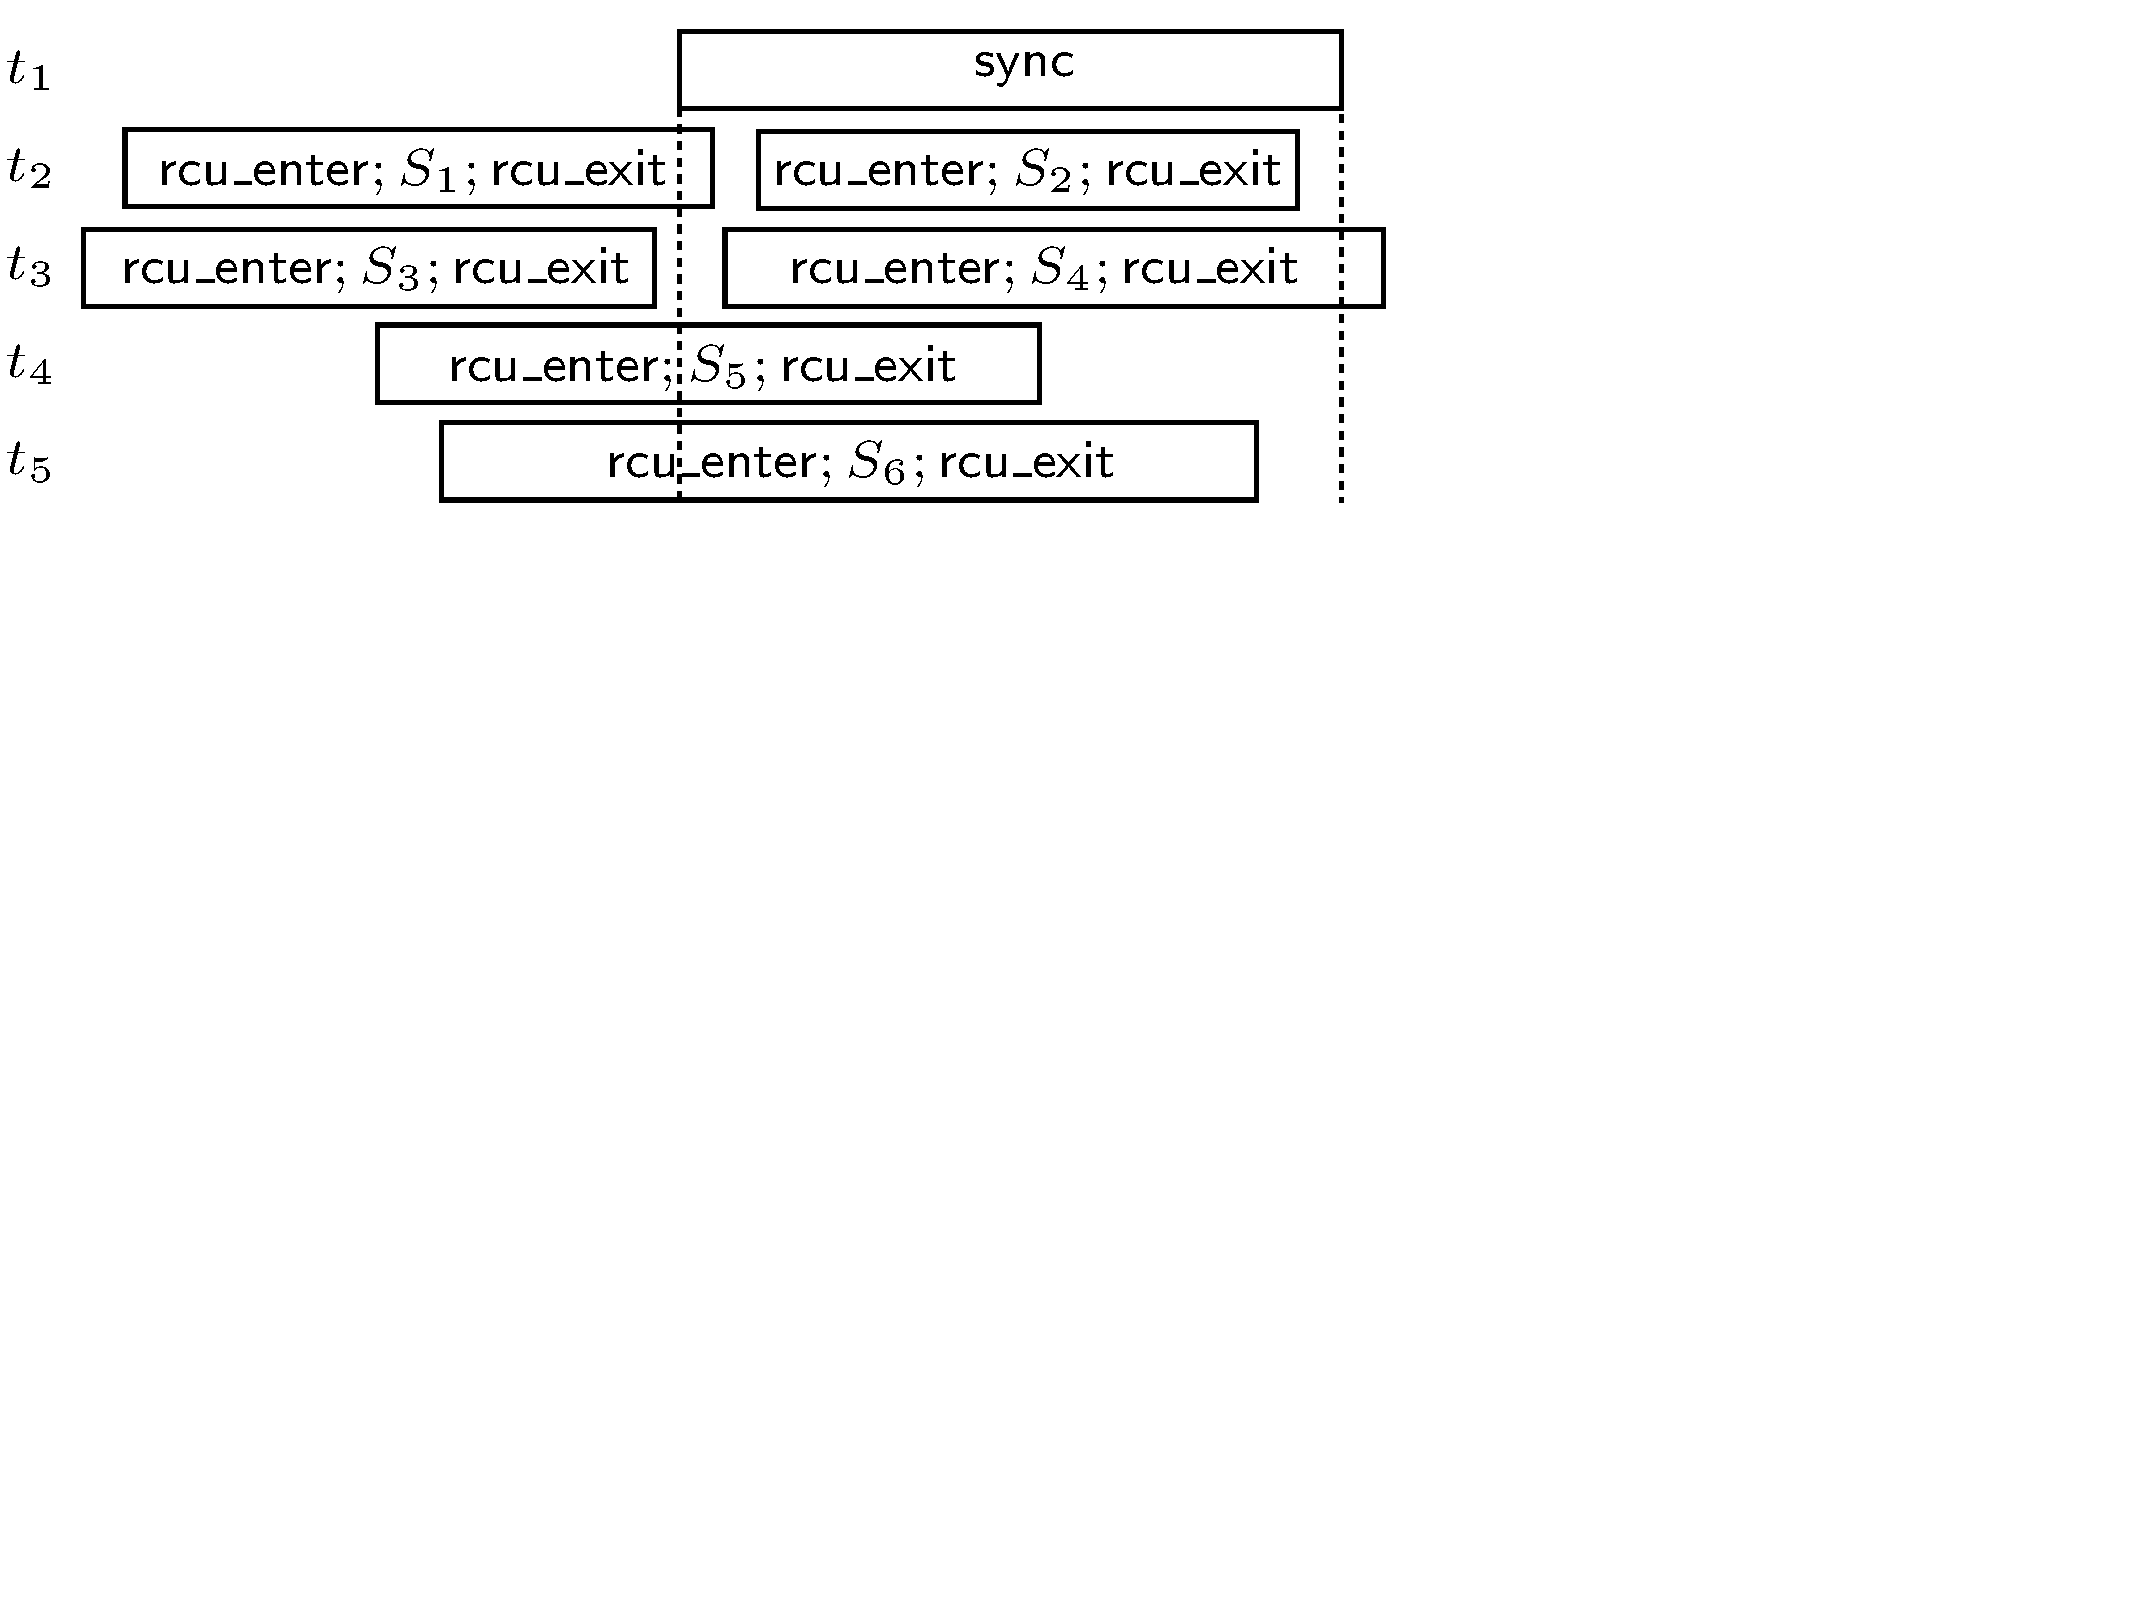
\includegraphics[scale=.27, trim= 0 18.5cm 0 0.1cm]{sync}
% \caption{An illustration of the semantics of $\sync$. Blocks represent the
%    time spans of RCU critical sections or an execution of $\sync$.}
%\label{fig:timeline}\label{fig:RCUProofSketch} 
%\end{figure}
%
%\begin{figure}[t]
%{\small
%\begin{lstlisting}[numbers=left, numberstyle=\tiny, language=C, escapeinside={(*}{*)}]
%bool rcu[N] = {0};
%rcu_enter() { (*$\langle$*)rcu[tid-1] = 1(*$\rangle_{\textsf{RCU}_\tid}$*); } 
%rcu_exit() { (*$\langle$*)rcu[tid-1] = 0(*$\rangle_{\textsf{RCU}_\tid}$*); } 
%sync() {
%  bool r[N] = {0};
%  for(int i = 0; i < N; i++) (*$\langle$*)r[i] = rcu[i](*$\rangle_{\textsf{Id}}$\label{impl:snap}*);
%  for(int i = 0; i < N; i++) if(r[i]) {while((*$\langle$*)rcu[i](*$\rangle_{\textsf{Id}}$\label{impl:wait}*));}
%}
%\end{lstlisting}
%}
%\label{fig:RCUProofSketch} 
%\caption{An abstract RCU implementation}
%\end{figure}
\begin{figure}[t]
\begin{center}
\begin{tabular}{@{\ }l@{\qquad\quad}|@{\qquad\qquad}l@{}}
{\figfontsize
\begin{lstlisting}[numbers=left, numberstyle=\tiny,language=C,escapeinside={(*}{*)}]
int *C = new int(0);
bool rcu[N] = {0};
Set detached[N] = {(*$\emptyset$*)};

void reclaim(int* s) {  
  insert(detached[tid-1], s);
  if (nondet()) return;
  sync();(*\label{rcua:sync}*)
  while (!isEmpty(detached[tid]))
     free(pop(detached[tid])); }
\end{lstlisting}}
&
{\figfontsize
\begin{lstlisting}[firstnumber=15,numbers=left, numberstyle=\tiny,language=C,escapeinside={(*}{*)}]
int inc() {
  int v, *n, *s;
  n = new int; rcu_enter();
  do {
    rcu_exit(); rcu_enter();
    s = C;(*\label{rcua:readc}*)  v = *s;(*\label{rcugeta:cderef}*) *n = v+1;
  } while (!CAS(&C,s,n));(*\label{rcua:cas}*)
  rcu_exit();
  reclaim(s);
  return v; }
\end{lstlisting}
}
\end{tabular}
\end{center}
\vspace{-5pt}
\caption{\label{fig:RCUCounter}
\small  Counter with RCU-based memory management}
\end{figure}

Figure~\ref{fig:RCUProofSketch} shows an {\em abstract} implementation of the
RCU primitives, formalising the above description of their semantics (for now,
the reader should disregard the annotations in the figure). A {\em concrete}
optimised RCU implementation would simulate the abstract one. Whether every
thread is inside or outside an RCU critical section is determined by its entry
in the {\tt rcu} array. 

%A thread should call $\sync$ only outside a critical section, as otherwise, it
%deadlocks.


\paragraph{RCU-based counter.}
Figure~\ref{fig:RCUCounter} gives the implementation of the running example
using RCU. Its overall structure is similar to the implementation using hazard
pointers. In {\tt inc}, we wrap an RCU critical section around the commands
starting from the read of the global variable $\cc$ at line~\ref{rcua:readc} and
including all memory accesses involving the value read up to the CAS at
line~\ref{rcua:cas}.  The correctness of the algorithm is ensured by having {\tt
  reclaim} call $\sync$ at line~\ref{rcua:sync}, before deallocating the
detached nodes. This blocks the thread until all critical sections that existed
at the time of the call to $\sync$ finish. Since, when $\sync$ is called, the
nodes to be deallocated have already been moved to the thread-local {\tt
  detached} set, newly arriving {\tt inc} operations have no way of gaining a
reference to one of these nodes, which guarantees the safety of their
deallocation. We can similarly argue that an ABA problem does not occur, and
thus, the algorithm is linearizable.  We can formulate the contract among
threads as follows:
% accessing nodes and those trying to reclaim them 
\be\label{rcu-inv} \mbox{
\begin{minipage}{10cm}
  ``for all $t$ and $x$, if thread $t$ has stayed in a critical section
  \underline{since} it saw $\cc$ pointing to $x$, then $x$ is allocated,''
\end{minipage}
} \ee 
which is of the same form as~(\ref{inf-inv}). Here, a grace period for a
thread, specified by the `since' clause, lasts for as long as the thread stays
in its critical section.
% \footnote{RCU papers~\cite{rcu-thesis} usually introduce
%   the grace period roughly as the time interval given by the negation of the `since'
%   clause, as formalised by~(\ref{rcu-neg}) below. In our setting, it is more
%   intuitive to organise the formalisation around the non-negated assertion.
% }
During the time span of $\sync$, every 
thread passes through a point when it is not in a critical section. Hence, after
executing line~\ref{rcua:sync}, for every node $x$ to be deallocated we know:
\be\label{rcu-neg} \mbox{
\begin{minipage}{10cm}
  ``for all $t$, $\cc$ has not pointed to $x$ \underline{since} $t$ was not in a
  critical section,''
\end{minipage}
}
\ee
which is of the same form as~(\ref{inf-neg}). As before,
this is inconsistent with the `since' clause of~(\ref{rcu-inv}), 
which guarantees that deallocating $x$ will not violate~(\ref{rcu-inv}).

\paragraph{Pattern.}
The algorithms using hazard pointers and read-copy-update fundamentally rely
on the same synchronisation pattern, where a potentially harmful race between
threads accessing nodes and those trying to reclaim them is avoided by
establishing an assertion of the form $(\eta_{t, x} \since \mu_x)$ before every
access, and $(\neg \mu_x \since \neg \eta_{t,x})$ before every deallocation.
This {\em implicit} pattern is highlighted not by examining the syntactic
structure of different memory management implementations, but by observing that
the arguments about their correctness have the same form,
as can be seen in our proofs. 
%In the rest of the paper, 
%We substantiate our claims by formalising the above reasoning in a logic and verifying the algorithms mentioned.



%%% Local Variables:
%%% TeX-master: "recycling"
%%% End:  
